\documentclass[10pt,letterpaper]{article}
\usepackage[margin=1in]{geometry}
\usepackage[T1]{fontenc}\usepackage{lmodern}
\usepackage[numbers,sort&compress]{natbib}
\usepackage{amsmath,amssymb,booktabs,graphicx,microtype,url,placeins,hyperref,xurl}
% Generated from saved results by tools/review_manuscript_artifacts.py.
\newcommand{\CTCFSequences}{51,249}
\newcommand{\UniqueSupport}{256,918}
\newcommand{\HitOccurrences}{281,915}
\newcommand{\FiniteTokens}{1,843,874}
\newcommand{\TokenRows}{1,946,372}
\newcommand{\AbsentSequences}{5,344}
\newcommand{\CaliperTATACount}{82}
\newcommand{\CaliperOtherCount}{456}
\newcommand{\CaliperDonorCount}{2,256}
\newcommand{\CaliperAcceptorCount}{2,352}
\newcommand{\HistoricalTATAPairs}{327}
\newcommand{\HistoricalTATATrain}{317}
\newcommand{\HistoricalTATATest}{10}
\newcommand{\BestQK}{0.3004}
\newcommand{\BestEnrichment}{1.3130}
\newcommand{\HeldoutTATAPairs}{10}
\newcommand{\NativePairs}{5,220}
\newcommand{\NativePositiveHeads}{58}
\newcommand{\NativeBestLayer}{6}
\newcommand{\NativeBestHead}{3}
\newcommand{\NativeBestContrast}{0.1471}
\newcommand{\NativeBestLow}{0.1317}
\newcommand{\NativeBestHigh}{0.1628}
\newcommand{\NativeBestHolm}{0.0144}
\newcommand{\SequenceQKPairs}{5,220}
\newcommand{\SequenceQKUndefined}{0}
\newcommand{\SequenceQKHighHeads}{0}
\newcommand{\SequenceQKBestLayer}{9}
\newcommand{\SequenceQKBestHead}{9}
\newcommand{\SequenceQKBestMean}{0.2595}
\newcommand{\SequenceQKBestLow}{0.2537}
\newcommand{\SequenceQKBestHigh}{0.2654}

\newcommand{\PerformanceTable}{%
\begin{tabular}{lrrr}
\toprule
Task & GC & $3$--$6$-mer & Frozen readout \\
\midrule
TATA promoter & 0.8955 [0.8496, 0.9337] & 0.9297 [0.8947, 0.9598] & 0.9136 [0.8748, 0.9476] \\
Other promoter & 0.9088 [0.8937, 0.9236] & 0.9406 [0.9292, 0.9517] & 0.9383 [0.9253, 0.9499] \\
Splice donor & 0.6560 [0.6375, 0.6750] & 0.8185 [0.8046, 0.8320] & 0.8954 [0.8838, 0.9059] \\
Splice acceptor & 0.6361 [0.6156, 0.6547] & 0.7956 [0.7792, 0.8113] & 0.8847 [0.8724, 0.8959] \\
\bottomrule
\end{tabular}
}

\newcommand{\ControlTable}{%
\begin{tabular}{lrrr}
\toprule
Task & Full & Historical matching & GC caliper \\
\midrule
TATA promoter & 0.9136 [0.8748, 0.9476] & 0.9136 [0.8738, 0.9477] & 0.7787 [0.6663, 0.8681] \\
Other promoter & 0.9383 [0.9253, 0.9499] & 0.9383 [0.9253, 0.9495] & 0.7254 [0.6796, 0.7710] \\
Splice donor & 0.8954 [0.8838, 0.9059] & 0.8943 [0.8826, 0.9054] & 0.8600 [0.8448, 0.8751] \\
Splice acceptor & 0.8847 [0.8724, 0.8959] & 0.8838 [0.8718, 0.8960] & 0.8607 [0.8457, 0.8750] \\
\bottomrule
\end{tabular}
}

\newcommand{\DatasetTable}{%
\begin{tabular}{lrrrr}
\toprule
Task & Train positive & Train negative & Test positive & Test negative \\
\midrule
TATA promoter & 2,531 & 2,531 & 106 & 106 \\
Other promoter & 14,980 & 15,020 & 686 & 686 \\
Splice donor & 15,084 & 14,916 & 1,480 & 1,520 \\
Splice acceptor & 15,031 & 14,969 & 1,475 & 1,525 \\
\bottomrule
\end{tabular}
}

\newcommand{\ThresholdTable}{%
\begin{tabular}{lrrrr}
\toprule
QK $r$ cutoff & Ratio $1.1$ & Ratio $1.25$ & Ratio $1.5$ & Ratio $2.0$ \\
\midrule
0.1 & 2 & 1 & 0 & 0 \\
0.2 & 0 & 0 & 0 & 0 \\
0.3 & 0 & 0 & 0 & 0 \\
0.4 & 0 & 0 & 0 & 0 \\
0.5 & 0 & 0 & 0 & 0 \\
\bottomrule
\end{tabular}
}

\newcommand{\PatchingTable}{%
\begin{tabular}{lrrrr}
\toprule
Layer/head & Mean PM & Median PM & Mean 95\% CI & Pairs \\
\midrule
2/7 & 0.3611 & 0.0306 & [-0.0265, 1.0250] & 10 \\
11/4 & 0.3118 & 0.0344 & [-0.1208, 0.9656] & 10 \\
3/10 & 0.2984 & 0.0385 & [0.0177, 0.6639] & 10 \\
\bottomrule
\end{tabular}
}

\newcommand{\SequenceQKTable}{%
\begin{tabular}{lrrr}
\toprule
Layer/head & Mean present $r$ [95\% CI] & Present--absent [95\% CI] & Holm $p$ \\
\midrule
9/9 & 0.2595 [0.2537, 0.2654] & -0.0539 [-0.0630, -0.0454] & 0.0144 \\
10/9 & 0.2085 [0.2026, 0.2143] & -0.0558 [-0.0632, -0.0476] & 0.0144 \\
7/2 & 0.2015 [0.1951, 0.2078] & 0.0103 [0.0018, 0.0183] & 0.7130 \\
\bottomrule
\end{tabular}
}

\title{MINTS supplementary evidence and reproduction}\author{Arjun VIjay Prakash\\Independent Researcher\\City Montessori School, Lucknow, India\\\texttt{arjunv.prakash12345@gmail.com}}\date{}
\begin{document}\maketitle
\section{Reporting revision and lineage}
Reporting revision v1 preserves original scientific protocols, memberships, outcomes and timestamps. The source archive is keyed to revision \path{cc09923652f0b361f73a36f382c4358dcf8b8100}; historical hardened receipts are checked against that source. Corrected summaries in \path{paper/figures} record original-input and new-generator hashes. Original run directories remain available.
\section{Corrected secondary dependence units}
Eleven non-primary scheme/direction tests form one secondary family per motif. The original ambiguous Holm column used sequence p-values. Named columns below correct sequence and block p-values over the same family. Block-based inference uses block Holm; primary CTCF block p remains 0.0028. Edits remain averaged within sequence. Clean/edited/sham exact/RC checks preserve 45 CTCF and 15 TATA held-out clusters.
\begin{table}[h]\centering\setlength{\tabcolsep}{4pt}\caption{Corrected secondary reporting from saved unadjusted p-values.}\begin{tabular}{lrrrr}
\toprule
Motif & Scheme & Direction & Sequence Holm & Block Holm \\
\midrule
TATA & all & denoise & 1.0000 & 1.0000 \\
TATA & all & reverse & 1.0000 & 1.0000 \\
TATA & all\_with\_special & denoise & 1.0000 & 1.0000 \\
TATA & all\_with\_special & reverse & 1.0000 & 1.0000 \\
TATA & edit & reverse & 1.0000 & 1.0000 \\
TATA & flank & denoise & 1.0000 & 1.0000 \\
TATA & flank & reverse & 1.0000 & 1.0000 \\
TATA & random & denoise & 1.0000 & 1.0000 \\
TATA & random & reverse & 1.0000 & 1.0000 \\
TATA & sparse & denoise & 1.0000 & 1.0000 \\
TATA & sparse & reverse & 1.0000 & 1.0000 \\
CTCF & all & denoise & 0.0180 & 0.0220 \\
CTCF & all & reverse & 0.1848 & 0.1337 \\
CTCF & all\_with\_special & denoise & 0.0143 & 0.0198 \\
CTCF & all\_with\_special & reverse & 1.0000 & 1.0000 \\
CTCF & edit & reverse & 0.1848 & 0.1434 \\
CTCF & flank & denoise & 1.0000 & 1.0000 \\
CTCF & flank & reverse & 1.0000 & 1.0000 \\
CTCF & random & denoise & 1.0000 & 1.0000 \\
CTCF & random & reverse & 1.0000 & 1.0000 \\
CTCF & sparse & denoise & 0.0297 & 0.0360 \\
CTCF & sparse & reverse & 0.1848 & 0.1256 \\
\bottomrule
\end{tabular}\end{table}\FloatBarrier
\section{Reviewer reproduction}
Pinned Python 3.14 CPU requirements support saved-evidence audits and reporting rebuilds without model or genome downloads. Public main and supplementary sources, diagnostics and generated inserts are available at \url{https://github.com/ArjunCodess/MINTS}. The historical diagnostic excerpt is versioned in \path{paper/diagnostic_scope.tex}; its original revision and all report-input hashes are recorded in \path{paper/figures/lineage.json}.
\begin{verbatim}
python -m pip install -r requirements-cpu.txt
python tools/audit_variant_study.py
python tools/audit_adastra_feasibility.py
python tools/audit_mapped_variant.py
python tools/check_query_correspondence.py
python tools/build_paper_artifacts.py
\end{verbatim}
Compile \path{main.tex} and \path{supplement.tex} with \texttt{latexmk -pdf} from \path{paper}. The correspondence example uses hand-constructed maps and tests contract behavior; it is not model calibration. Sequence-free reproduction data and all 61 unchanged native logit files are publicly archived at \url{https://doi.org/10.5281/zenodo.23267982}. Extract the dataset ZIP into \texttt{DATA\_DIR} and run the verifier from the public code checkout:
\begin{verbatim}
python tools/verify_deposit.py --data-root DATA_DIR
\end{verbatim}
The verifier checks the deposited file hashes, all raw divergences, headline estimates and uncertainty, secondary Holm reporting and overall sensitivity corrections. It uses saved cluster assignments. Reconstructing sequence-aware clusters, eligibility, source inputs or fresh inference requires the pinned upstream resources and their terms. The private mixed-resource reviewer archive is not the public dataset.
Full scientific execution requires the pinned tokenizer/checkpoint, verified native weights, genome, intervals and residual caches. It is unnecessary for report reproduction. Extensions require separately frozen protocols. Windows CPU validation and historical Windows CUDA execution differ from Linux CI; no new Linux scientific run is asserted. Original code is MIT and original scientific outputs are CC-BY-4.0. Third-party data and model resources retain their own terms; these grants do not resolve absent dataset or checkpoint permissions.
\section{Diagnostic context}
The following material preserves historical failures, alternative aggregation, cohort balance and provenance limitations. Withdrawn patch rankings are diagnostic; fixture calibration is limited to engineered computations. The sensitivity table now shows both corrections. Secondary block interpretation is superseded by the corrected table above. These diagnostics do not reopen stopped studies.
% Historical diagnostic excerpt from cc09923652f0b361f73a36f382c4358dcf8b8100:paper/main.tex.
\section{Datasets and audit scope}
We use locally saved partitions of \path{InstaDeepAI/nucleotide_transformer_downstream_tasks_revised}, filtering the task field and retaining sequence, coordinate name, and binary label. Saved data have train and test partitions, with no independent validation partition. Test examples are on chromosomes 20 and 21; training examples are on chromosomes 1--19, X, and Y. Table~\ref{tab:dataset} gives exact class counts. The original run did not pin an upstream revision. New ingestion pins \path{851f9946252e90c665cdb3cc3eedb78f1f26197c}; its official card URL, content hash, and label-source URLs are saved with the audit.

The released card attributes promoter labels to EPDnew human release 006, using promoter intervals and its TATA motif annotation, with genomic non-promoter windows as negatives. It attributes splice labels to GENCODE human release 44, excluding level-3 transcript annotations. We use the released labels without resampling or changing windows. The card documents promoter source filenames and splice annotation release, but does not give every sampling decision needed to independently reconstruct all labels. Membership hashes establish analyzed examples, rather than certifying the biological annotations.

Ordered hashes of labels, coordinates, sequences, and tokenization agree exactly between the stored partitions and fresh ingestion of the pinned release for all four tasks. This verifies the analyzed dataset against that release, without recovering historical checkpoint provenance or independently validating its labels.
\begin{table}[t]
\centering\normalsize
\caption{Exact stored class counts. Membership, coordinates, sequence hashes, and orientation-canonical hashes are saved as JSONL.}
\label{tab:dataset}
\DatasetTable
\end{table}

Checks find no shared chromosomes, overlapping windows, identical sequences, or reverse-complement duplicates across stored train/test partitions. An exhaustive equal-length Hamming screen finds no cross-partition pair with at most two substitutions in either orientation. This does not cover indels, shifted windows, or longer-range homology. No reverse-complement augmentation is introduced. Chromosome-held-out evaluation cannot rule out reference-genome overlap in pretraining.

CTCF sequences come from ENCODE experiment ENCSR000DKV, peak file ENCFF827JRI, and the UCSC hg38 reference. BED intervals are extracted without flanks; the prepared file contains \CTCFSequences{} intervals. Peaks are assay observations rather than proof of a particular motif or a model's binding prediction. Local source hashes are audited. New inference pins the model revision stated above; the historical unpinned checkpoint cannot be reconstructed from these hashes alone.

\section{Results}
\paragraph{The audit separates evidence that supports different claims.}
Decodable labels and conditional attention associations do not establish causal motif use. Historical patching has broken nucleotide alignment and unstable restoration ratios. The fitted CTCF baseline-plus-residual classifier has a negative incremental comparison on the analyzed population; it does not prove absence of additional representational information. The repaired trained-readout intervention uses 64 sequences in 45 genomic clusters. Its target remains a fitted readout, so these measurements cannot establish a native biological binding mechanism. Individual-head screen failures also leave distributed mechanisms unresolved.
\paragraph{Prediction is context, not a mechanism.}
Table~\ref{tab:task-performance} shows higher point AUROC for the k-mer classifier than the DNABERT-2 readout on both promoter tasks; this is not a claim of statistically established superiority. The readout has higher point AUROC on splice tasks. Strong promoter composition baselines make a motif-specific explanation especially uncertain.
\begin{table}[t]
\centering\normalsize\setlength{\tabcolsep}{3pt}
\caption{Held-out AUROC with 95\% sequence-bootstrap intervals, generated from saved per-sequence predictions.}
\label{tab:task-performance}
\PerformanceTable
\end{table}

\paragraph{Composition matching changes the promoter result.}
Table~\ref{tab:probe-controls} retains the historical match for auditability and compares the repaired caliper control. Historical and full promoter AUROC legitimately agree for identical memberships, but this provides no composition control. Historical splice subsets are smaller and their AUROCs differ from full scores. The caliper retains \CaliperTATACount{} examples in the TATA task, \CaliperOtherCount{} in the other-promoter task, \CaliperDonorCount{} in the donor task, and \CaliperAcceptorCount{} in the acceptor task. On these retained populations, promoter readout AUROC is lower and the GC baseline approaches chance. Because matching selects a different population, the AUROC change does not isolate an effect of GC. This supports a narrower promoter interpretation and does not establish causal motif use.
\begin{table}[t]
\centering\normalsize\setlength{\tabcolsep}{3pt}
\caption{Readout AUROC and 95\% sequence-bootstrap intervals. Full, historical, and caliper populations differ; retained counts and composition diagnostics accompany the predictions.}
\label{tab:probe-controls}
\ControlTable
\end{table}

\paragraph{CTCF screen failure is scoped to this assay.}
The token-score file has \TokenRows{} rows, including \FiniteTokens{} finite scores and \UniqueSupport{} unique motif-support tokens. Summing participation separately over overlapping hits gives \HitOccurrences{} motif-hit token occurrences, the quantity used by historical enrichment. There are \AbsentSequences{} peaks without a threshold-passing PWM hit. These count different filtering and aggregation stages.

The maximum historical QK correlation is \BestQK{} and reconstructed enrichment ratio is \BestEnrichment{}. No head passed the motif-local QK and attention-enrichment screens. Table~\ref{tab:sweep} gives the joint sweep from saved head tables. This does not establish absence of a CTCF detector. We withdraw inferential interpretations of old token-shuffle and permuted-head nulls, which do not provide sequence-level evidence for localization.
\begin{table}[t]
\centering\normalsize
\caption{Heads passing both descriptive cutoffs in the historical reconstructed-attention assay. No significance or confidence interval is assigned to a count of screened heads.}
\label{tab:sweep}
\ThresholdTable
\end{table}

\paragraph{Native attention associates with motif-present peaks.}
The separate genomic-control assay retains \NativePairs{} pairs, with no invalid pairs. Reconstructed and native head contexts agree to the measured precision (maximum absolute error zero). There are \NativePositiveHeads{} heads with positive contrasts and Holm-adjusted $p<0.05$. The largest mean contrast, layer/head \NativeBestLayer{}/\NativeBestHead{}, is \NativeBestContrast{} (marginal 95\% interval [\NativeBestLow{}, \NativeBestHigh{}]; Holm $p=\NativeBestHolm{}$). Figure~\ref{fig:native} shows the largest observed contrasts. These conditional associations qualify the historical negative result, but do not supply a native causal output. Selection of displayed maxima is exploratory.
\begin{figure}[t]
\centering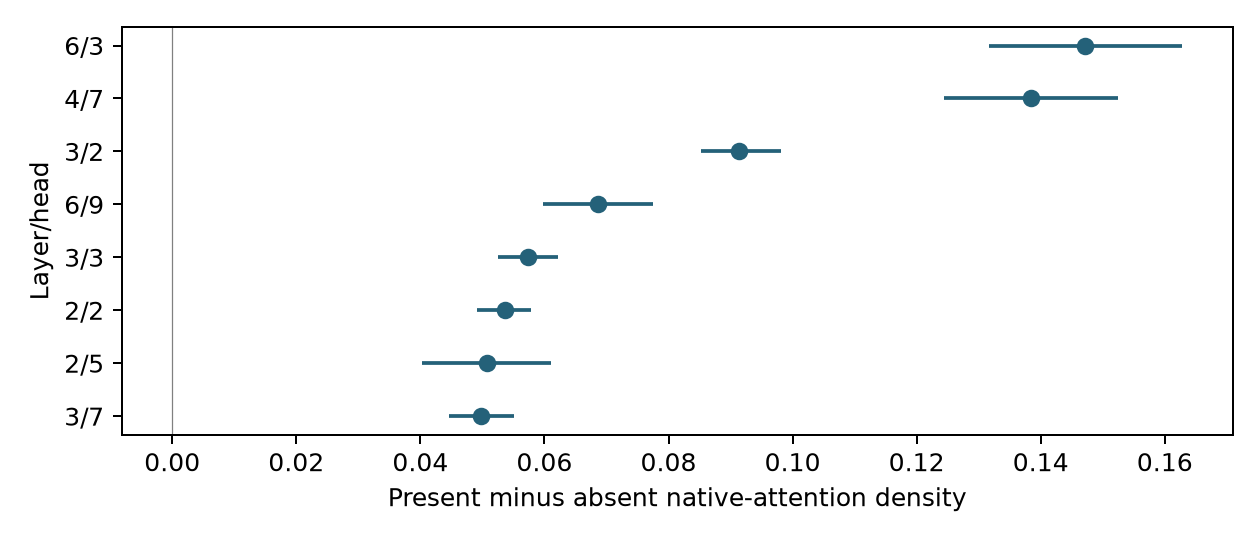
\includegraphics[width=.9\linewidth]{../results/review/ctcf_native_controls.png}
\caption{Native-attention density contrasts for the eight largest observed means. Intervals bootstrap matched sequence pairs and are marginal; tests correct across all 144 heads.}
\label{fig:native}
\end{figure}

\paragraph{Sequence-level QK is a separate localization assay.}
The sequence-level QK analysis retains \SequenceQKPairs{} matched pairs; \SequenceQKUndefined{} pairs have undefined correlations. The largest mean motif-present correlation is \SequenceQKBestMean{} at layer/head \SequenceQKBestLayer{}/\SequenceQKBestHead{} (marginal 95\% interval [\SequenceQKBestLow{}, \SequenceQKBestHigh{}]). There are \SequenceQKHighHeads{} heads with mean $r\geq0.5$. Table~\ref{tab:sequence-qk} shows the largest observed means and their matched contrasts. The two heads with the largest mean present correlations have negative present--absent contrasts: their mean correlations are higher in motif-absent peaks. Positive within-sequence correlation alone therefore does not imply selective association with threshold-passing motifs. This is a new sequence-weighted content-QK assay, so it does not replace the pooled historical statistic or establish causal use.
\begin{table}[t]
\centering\normalsize\setlength{\tabcolsep}{3pt}
\caption{Exploratory sequence-level QK means and contrasts. Intervals bootstrap sequence pairs; two-sided contrast tests use a separate Holm family of 144 heads. Displayed heads are selected by observed mean present correlation.}
\label{tab:sequence-qk}
\SequenceQKTable
\end{table}

\paragraph{Historical held-out patching is withdrawn as aligned evidence.}
The earlier \HistoricalTATAPairs{} TATA pairs contain \HistoricalTATATrain{} training and \HistoricalTATATest{} test examples, with unique pair IDs; pooling partitions explains the apparent excess over the test-set size. That pooled effect is withdrawn as held-out causal evidence. The archived test-only results retain \HeldoutTATAPairs{} shape-compatible examples, six with nucleotide-boundary mismatches at patched positions. Table~\ref{tab:patching} reports the largest mean effects with medians and marginal intervals. Figure~\ref{fig:pairs} shows individual pairs and their denominators. Sign changes in the reference difference and variation across pairs limit interpretation of the mean ratio. The intervention changes a trained readout and cannot certify a biological detector in the pretrained model.
\begin{table}[t]
\centering\normalsize
\caption{Archived TATA probe patching, withdrawn as aligned intervention evidence and retained for diagnosis, ranked by mean PM. Intervals bootstrap pairs and are marginal, without correction for choosing maxima across 144 heads.}
\label{tab:patching}
\PatchingTable
\end{table}
\begin{figure}[t]
\centering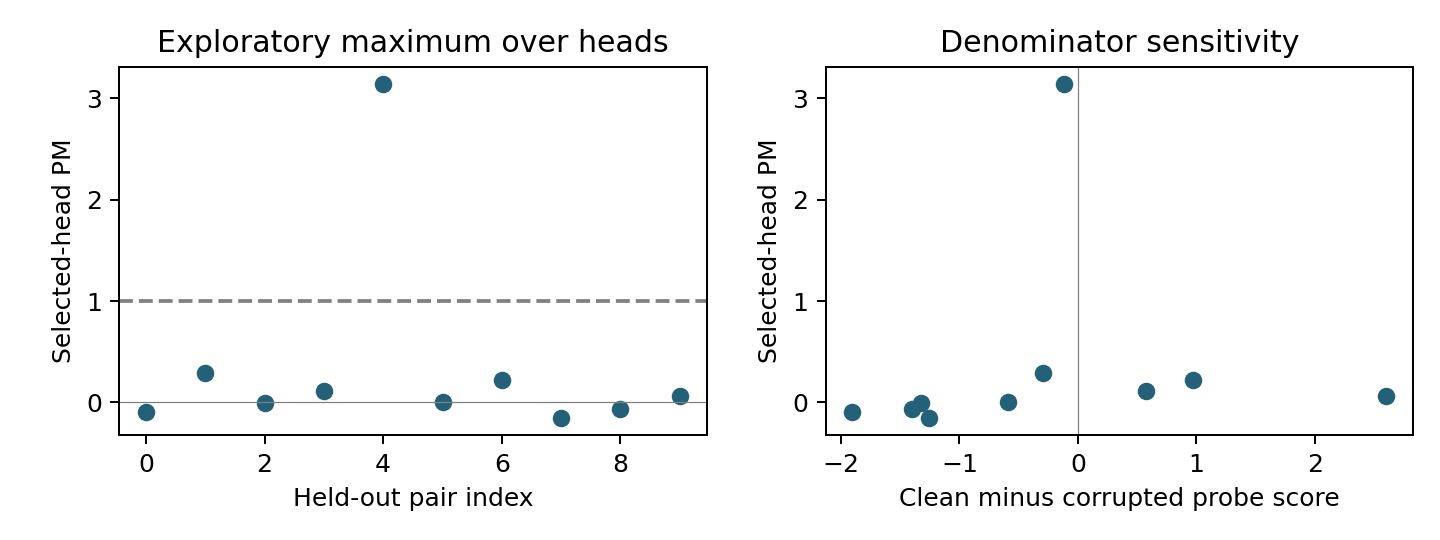
\includegraphics[width=\linewidth]{../results/review/heldout_patching.png}
\caption{Pair PM for the head with the largest observed mean, and its clean-corrupted score difference. Selection is exploratory.}
\label{fig:pairs}
\end{figure}

\FloatBarrier
% Generated from validated hardened stage artifacts.

\section{Engineered calibration and held-out trained-readout assays}

\paragraph{Known-mechanism calibration.}

Oracle motif features implanted in QK and V span TATA and CTCF, single-head, query-specific, distributed, composition-only, and randomized computations. Strength, position, and instance count vary. Thresholds chosen on discovery seeds yield confirmation sensitivity 1.000 and false-positive rate 0.000. This validates engineered base-token fixtures, not sensitivity to learned DNABERT mechanisms.

\begin{figure}[t]\centering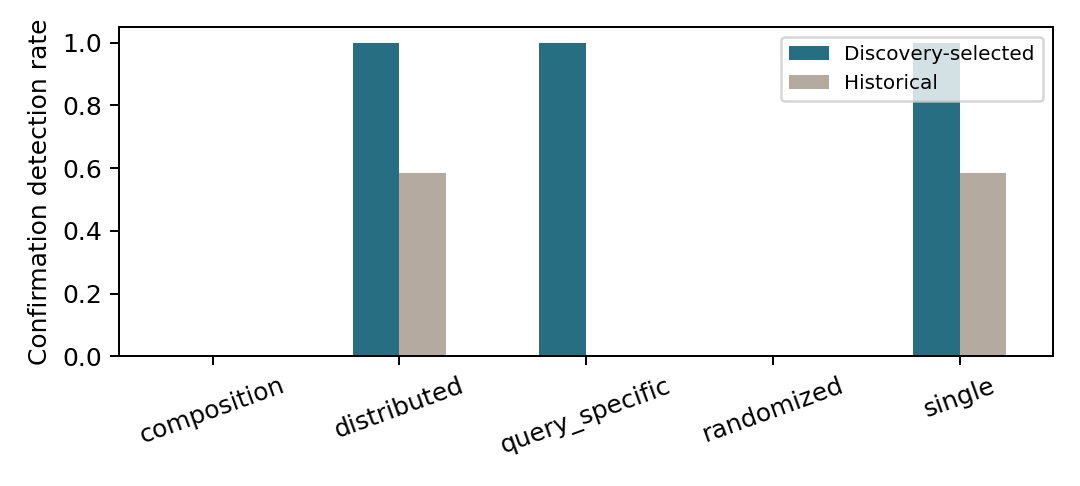
\includegraphics[width=.85\linewidth]{../results/hardened/figures/calibration.png}\caption{Oracle fixture calibration on separate fixture seeds; per-observation head selection does not calibrate natural-data selection.}\end{figure}

\paragraph{Incremental prediction.}

Baseline features include mono- and dinucleotide composition, motif count, score and relative position, and window coordinates. Baseline-only and baseline-plus-residual models use identical populations, validation-selected regularization, and fixed held-out predictions. Table~\ref{tab:incremental} gives paired 1 Mb genomic-block intervals.

\begin{table}[t]\centering\normalsize\caption{Baseline-plus-residual minus baseline-only AUROC.}\label{tab:incremental}

\begin{tabular}{lrrr}
\toprule
Task & $\Delta$ AUROC & 95\% block interval & Clusters \\
\midrule
TATA & 0.0412 & [0.0111, 0.0678] & 87 \\
Other promoter & 0.0240 & [0.0137, 0.0352] & 107 \\
Donor & 0.2089 & [0.1814, 0.2385] & 107 \\
Acceptor & 0.2360 & [0.2024, 0.2670] & 107 \\
Accessible CTCF & -0.0454 & [-0.0756, -0.0166] & 81 \\
\bottomrule
\end{tabular}

\end{table}

\paragraph{Aligned composition controls.}

Motif and sham edits preserve exact A/C/G/T counts and match nucleotide transitions, edit count, window width, overlapping BPE count, and covered nucleotide width. Shams occupy the nearest eligible non-motif window, with distance logged. All token boundaries agree, the target motif is destroyed, and no new threshold-passing hit locations are created. Eligibility uses sequence properties without output filtering. Six of ten historical TATA pairs have incompatible boundaries at patched positions; their PM rankings are withdrawn as aligned intervention evidence.

Discovery on chromosomes 18/19 chooses one of 144 heads, whose identity and scorer are frozen before confirmation on 20/21. Absolute motif-minus-sham score changes are primary. Edits are averaged within sequence; genomic blocks merge shared intervals and exact or reverse-complement inputs. Discovery carries simultaneous maximum-statistic inference. Confirmation saves individual scores, leave-one-out estimates, and six schemes in both denoising and reverse directions. The original secondary column used sequence Holm. Reporting revision v1 below supplies both dependence units; block Holm governs block-based interpretation. Donor GT edits retain insufficient aligned matched examples, so no donor mechanism is inferred.

\begin{table}[t]\centering\normalsize\caption{Fixed-head trained-readout intervention on held-out chromosomes.}\label{tab:controlled}

\begin{tabular}{lrrrrr}
\toprule
Motif & Head & Sequences & Effect & 95\% block interval & $p$ \\
\midrule
TATA & 0/8 & 16 & 0.0243 & [-0.0338, 0.1014] & 0.5772 \\
CTCF & 5/8 & 64 & 0.0157 & [0.0066, 0.0251] & 0.0028 \\
\bottomrule
\end{tabular}

\end{table}

\begin{figure}[t]\centering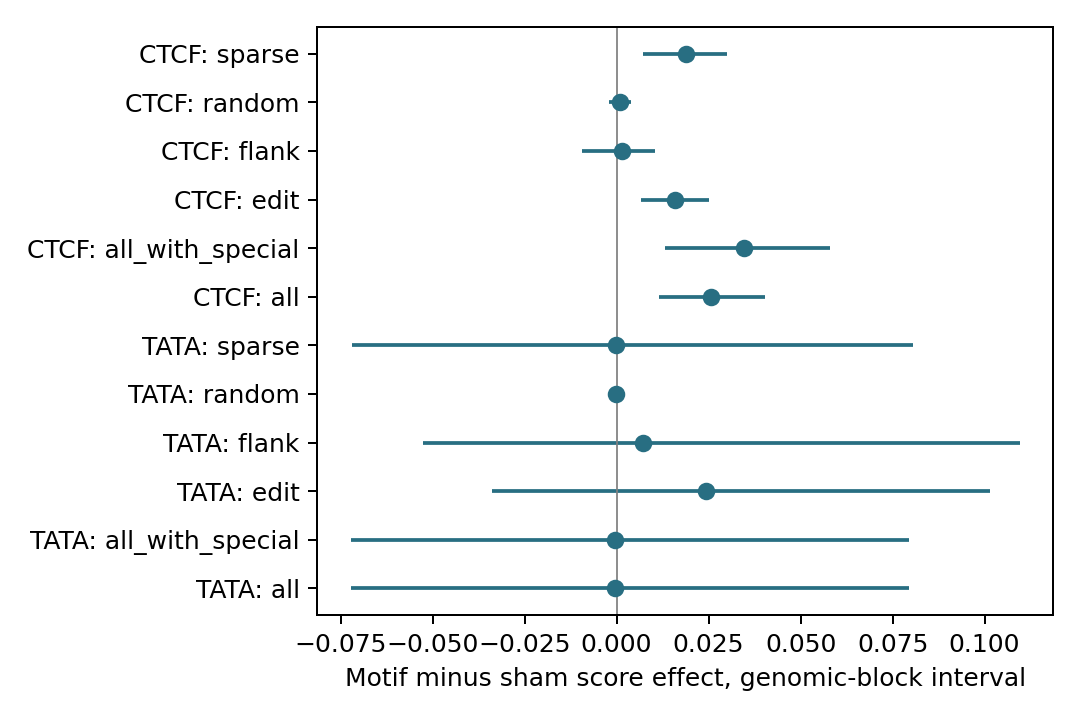
\includegraphics[width=.9\linewidth]{../results/hardened/figures/controlled_interventions.png}\caption{Genomic-block intervals for fixed-head denoising schemes; secondary schemes are exploratory.}\end{figure}

\paragraph{Independent accessible CTCF cohort.}

GM12878 DNase experiment ENCSR000EMT, GRCh38 file ENCFF598KWZ, defines accessible windows independently of the saved CTCF peaks. Cases overlap those peaks; controls do not, including motif-bearing non-overlap windows. Matching uses chromosome, 204 bp width, GC within 0.02, and log-DNase signal within 0.5. Per-class caps are 512 training, 128 validation, and 128 test. The readout passes its pre-execution validation AUROC gate of 0.6 with validation AUROC 0.6859 and test AUROC 0.6699. Localization and intervention use the same CTCF motif and trained output. The paired incremental comparison in Table~\ref{tab:incremental} is negative for CTCF: this fitted concatenation underperforms the fitted direct baseline, without establishing absence of extra representational information. Peak non-overlap does not verify binding absence. Repeat annotations, quantitative occupancy, and other cell types are unavailable.

\paragraph{Native attention sensitivity.}

PWM score-range fractions 0.7, 0.8, and 0.9 recompute scoring and matching across 51,249 peaks. Each configuration evaluates at most 256 random eligible pairs. Token balancing requires identical real-token and target-token counts and covered widths within 2 bp. Maximum, mean, and overlap-weighted aggregation give separate QK assays. Attention compares base and token weighting, global and local queries, and native, content-only, and position-only softmax. Every native head context is checked. Table~\ref{tab:geometry} counts positive base-density contrasts passing genomic-block maximum-statistic tests over 144 heads; saved inference also corrects across all sensitivity choices and reports chromosome effects.

\begin{table}[t]\centering\caption{Sensitivity counts under both saved families. Within uses 144-head maximum-statistic tests; overall Holm includes all metrics, thresholds, geometries, heads and both resampling summaries.}\label{tab:geometry}\begin{tabular}{lrrrrr}
\toprule
Fraction & Geometry & Eligible & Scored & Within & Overall \\
\midrule
0.70 & nucleotide\_matched & 82 & 82 & 0 & 0 \\
0.70 & token\_balanced & 15 & 15 & 1 & 0 \\
0.80 & nucleotide\_matched & 5220 & 256 & 7 & 0 \\
0.80 & token\_balanced & 3510 & 256 & 44 & 0 \\
0.90 & nucleotide\_matched & 13090 & 256 & 12 & 0 \\
0.90 & token\_balanced & 5088 & 256 & 55 & 0 \\
\bottomrule
\end{tabular}\end{table}

\paragraph{Scope and reproducibility.}

These experiments test computational calibration and trained-readout effects without establishing native pretrained binding causality. Protocol choices precede execution without external registration. Distant homology, label reconstruction, pretraining exposure, and classifier-seed variability remain unresolved. Immutable legacy-pipeline receipts reject changed scientific configuration, source, membership, or artifacts on resume. Isolated execution records retain prior receipts and verify source and artifact hashes before generating these results.

\paragraph{Additional descriptive balance audit.}
Normalized BED scores are available in the prepared CTCF peaks, although quantitative occupancy and repeat annotations are not. Table~\ref{tab:bed-balance} reports their means in evaluated native-control pairs. Matching does not constrain this score, so differences remain possible confounders. Most peaks reach the score ceiling of 1000. Saved diagnostics also report base entropy, longest mononucleotide runs, and DNase balance by motif presence and partition; these sequence-complexity measures do not identify repeat annotations. This post-hoc audit does not select heads or modify inference.
\begin{table}[t]\centering\normalsize\caption{Normalized CTCF BED-score balance in evaluated pairs.}\label{tab:bed-balance}
\begin{tabular}{lrr}\toprule Configuration & Present mean & Absent mean \\\midrule
f0.70\_nucleotide\_matched\_pairs & 1000.0 & 941.6 \\
f0.70\_token\_balanced\_pairs & 954.2 & 796.5 \\
f0.80\_nucleotide\_matched\_pairs & 994.9 & 894.8 \\
f0.80\_token\_balanced\_pairs & 940.9 & 909.9 \\
f0.90\_nucleotide\_matched\_pairs & 981.9 & 964.9 \\
f0.90\_token\_balanced\_pairs & 982.8 & 947.8 \\
\bottomrule\end{tabular}
\end{table}

\paragraph{Discovery-only native masked-flank pilot.}
A separate fixed-endpoint pilot loads the pinned pretrained masked-language-model head without fitting a readout. No prediction-head parameters are missing or newly initialized. The target is the nearest unchanged whole downstream flank token at a gap of 1--30 bases, with upstream fallback. Its nucleotide span and token identity agree across clean, composition-preserving motif-edited and transition-matched sham sequences, and masking leaves the motif edit visible. On chromosomes 18/19, 12 retained sequences form 11 transitive genomic clusters. The mean motif-minus-sham target log-probability loss is $-0.0568$ nats with a 95\% cluster interval $[-0.2513, 0.0869]$. This fails the prespecified feasibility requirement of at least eight clusters, a positive interval lower bound and a mean of at least 0.05 nats. We stop before head selection or confirmation, rather than search other outputs. The interval is too wide to establish a precise null. This result concerns the chosen sequence-prediction endpoint; it does not establish absence of a CTCF mechanism. The already inspected chromosomes 20/21 cannot supply fresh confirmation for any subsequent extension.

\paragraph{Endpoint and control diagnostics.}
A separate exploratory follow-up holds the original motif edit and target fixed and requires a same-side sham within two bases of the motif-to-target distance, preserving window width and token geometry. Two disjoint 19-base windows on the same side must differ in target distance by at least 19 bases. Thus none of the 12 original pairs has a feasible tightly matched same-sequence control. We record this exclusion without relaxing the tolerance or claiming a revised motif effect. Removing one entire genomic cluster moves the original mean contrast from $-0.0922$ to $0.0163$ nats, including a sign change. Eligibility metrics cover all 21 scanned sequences, including the 12 retained examples.

\paragraph{Native recovery and intervention controls.}
A fixed population of 128 windows on chromosomes 16/17 masks one seeded random real token per window, without using model outcomes for selection. Token frequencies are estimated separately on chromosomes 14/15. Median correct-token rank is 57.5, top-1 recovery is 6.25\%, and mean target log probability is -6.0632 nats versus -6.8769 for the smoothed frequency baseline. These descriptive results show recovery utility on that population, without establishing motif-specific endpoint sensitivity. Identity context patches, complete final-residual rescue and reverse controls pass in all 24 motif/sham cases. Final-residual replacement includes the residual bypass; attention-only recovery is recorded separately. An engineered motif-dependent predictor also passes a known-mechanism rescue check through the same hook interface.

\paragraph{An independently measured allele benchmark is recoverable.}
The published supplemental Table S3 for GSE81945 supplies 16 mutation rows with pooled WGS and CTCF ChIP counts \citep{poulos2016ctcf}. Its reference alleles agree with UCSC hg19 at the listed one-based positions. There are 15 heterozygous variants in 13 locus groups; one homozygous row cannot identify a normalized allele effect. Two groups contain adjacent variants with unresolved phase. Input-normalized effects and descriptive half-count log-odds intervals are saved, but pooled counts cannot recover replicate variation or mapping-bias uncertainty. This small selected benchmark lacks substitution-matched controls and does not supply fresh biological confirmation.

% Generated by tools/build_mapped_report.py from audited frozen evidence.
\subsection{Expanded natural-variant diagnostic and mapped-query study}
The archived ADASTRA Mabel v6.1 CTCF table \citep{adastra2024release,abramov2021adastra} contains 512,556 coverage-eligible
records, including nonsignificant records. A prior 4,096-case hash screen retained
no strict controls. A separately frozen exploratory expansion to 12,288 verified
hg38 single-SNV reference scenarios retained one strict control in the added 8,192
cases. Complete allele BPE offsets agree in 4,850 cases; exact local query spans
and token identities exist in all 12,288. Reference motifs cover 433 variants.
Same-side query distance differences equal edit separation, making the 16-base
tolerance more restrictive than the nominal 64-base sham search. Independent
candidate predicates and their intersections diagnose attrition without changing
the original sequential eligibility decisions.

A new exploratory protocol removes complete input-offset and edit-token-width
matching while retaining exact query correspondence, substitution, trinucleotide,
GC, motif preservation and 16-base geometry controls. It retains 61 cases in 60
genomic/sequence proxy clusters. Query indices are explicitly mapped, and 29 cases
change an index. Each unchanged query is masked separately with both edits visible;
Jensen--Shannon divergence is weighted by nucleotide width. Native identity, repeat,
mapped final-query restoration and reverse restoration pass implementation checks.
The pointwise MLM head makes final-query representation restoration an exact
logit-recovery control; no such requirement is imposed on individual heads.

Variant and sham mean divergences are 0.013053
and 0.029018 nats. The equal-cluster contrast is
-0.015966, with 95\% bootstrap interval
[-0.024454, -0.009146]. The shams perturb predictions more,
failing the positive differential-sensitivity gate. Every leave-cluster-out mean
remains negative; chromosome aggregation also remains negative. The width-matched
11-cluster subset has contrast -0.006758 with interval
[-0.014121, 0.000623]. Its Holm p-value
is 0.2443; absolute PWM-change agreement has Spearman
rho 0.1428, Holm p=0.2763.
Fifteen boundary-stable triplets all have negative contrasts, a descriptive
post-inspection diagnostic rather than a new confirmation test.

This result concerns generic native prediction sensitivity on a small matchable
population. It does not identify binding direction, absent variant sensitivity,
or a causal CTCF mechanism. Segmentation, positional effects, sequence context,
indirect binding and selected-population effects remain plausible alternatives.
ADASTRA weighted log2 observed/expected effects are not interchangeable with
GSE81945 input-normalized log odds. Live provenance retrieval exposes 238 ChIP
allele-count observations for 26 cases across 174 experiments, but only five
components after joining shared experiments. Donor/phase, per-replicate input,
mapping correction and dosage uncertainty remain unverified. Biological QC
therefore fails separately from native sensitivity. No biological correlation,
head discovery, intervention-based power or independent confirmation is run.
Earlier stopped protocols and results remain intact.

\begin{figure}[t]
\centering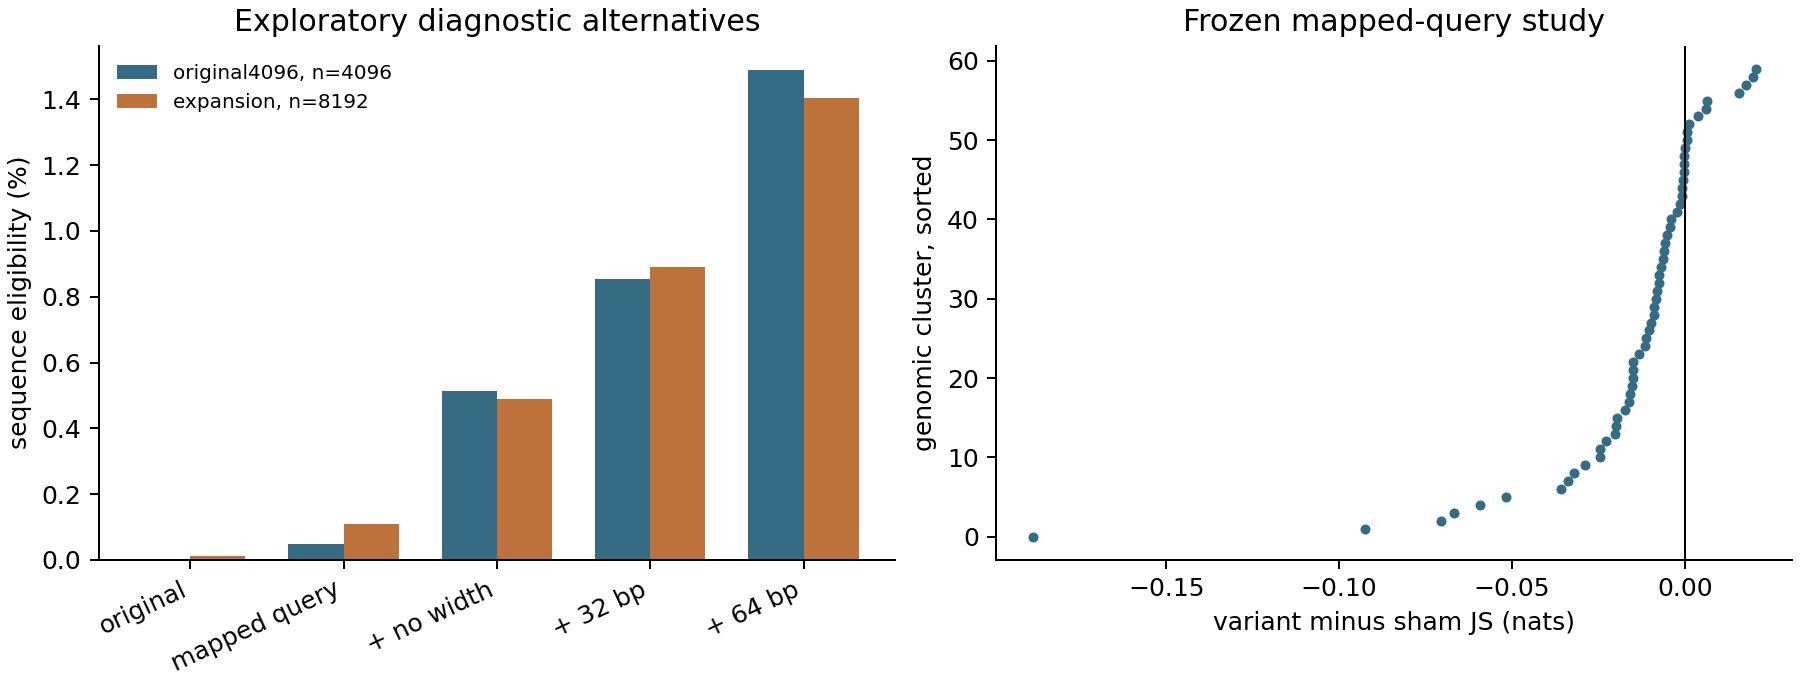
\includegraphics[width=\linewidth]{../results/mapped_variant/report/study.png}
\caption{Sequence-only diagnostic retention under declared alternatives and
cluster-level native contrasts under the separately frozen mapped-query design.
Alternatives were examined before scoring and are exploratory. Genomic clusters
are dependence proxies, not verified independent donors.}
\end{figure}

\begin{figure}[t]
\centering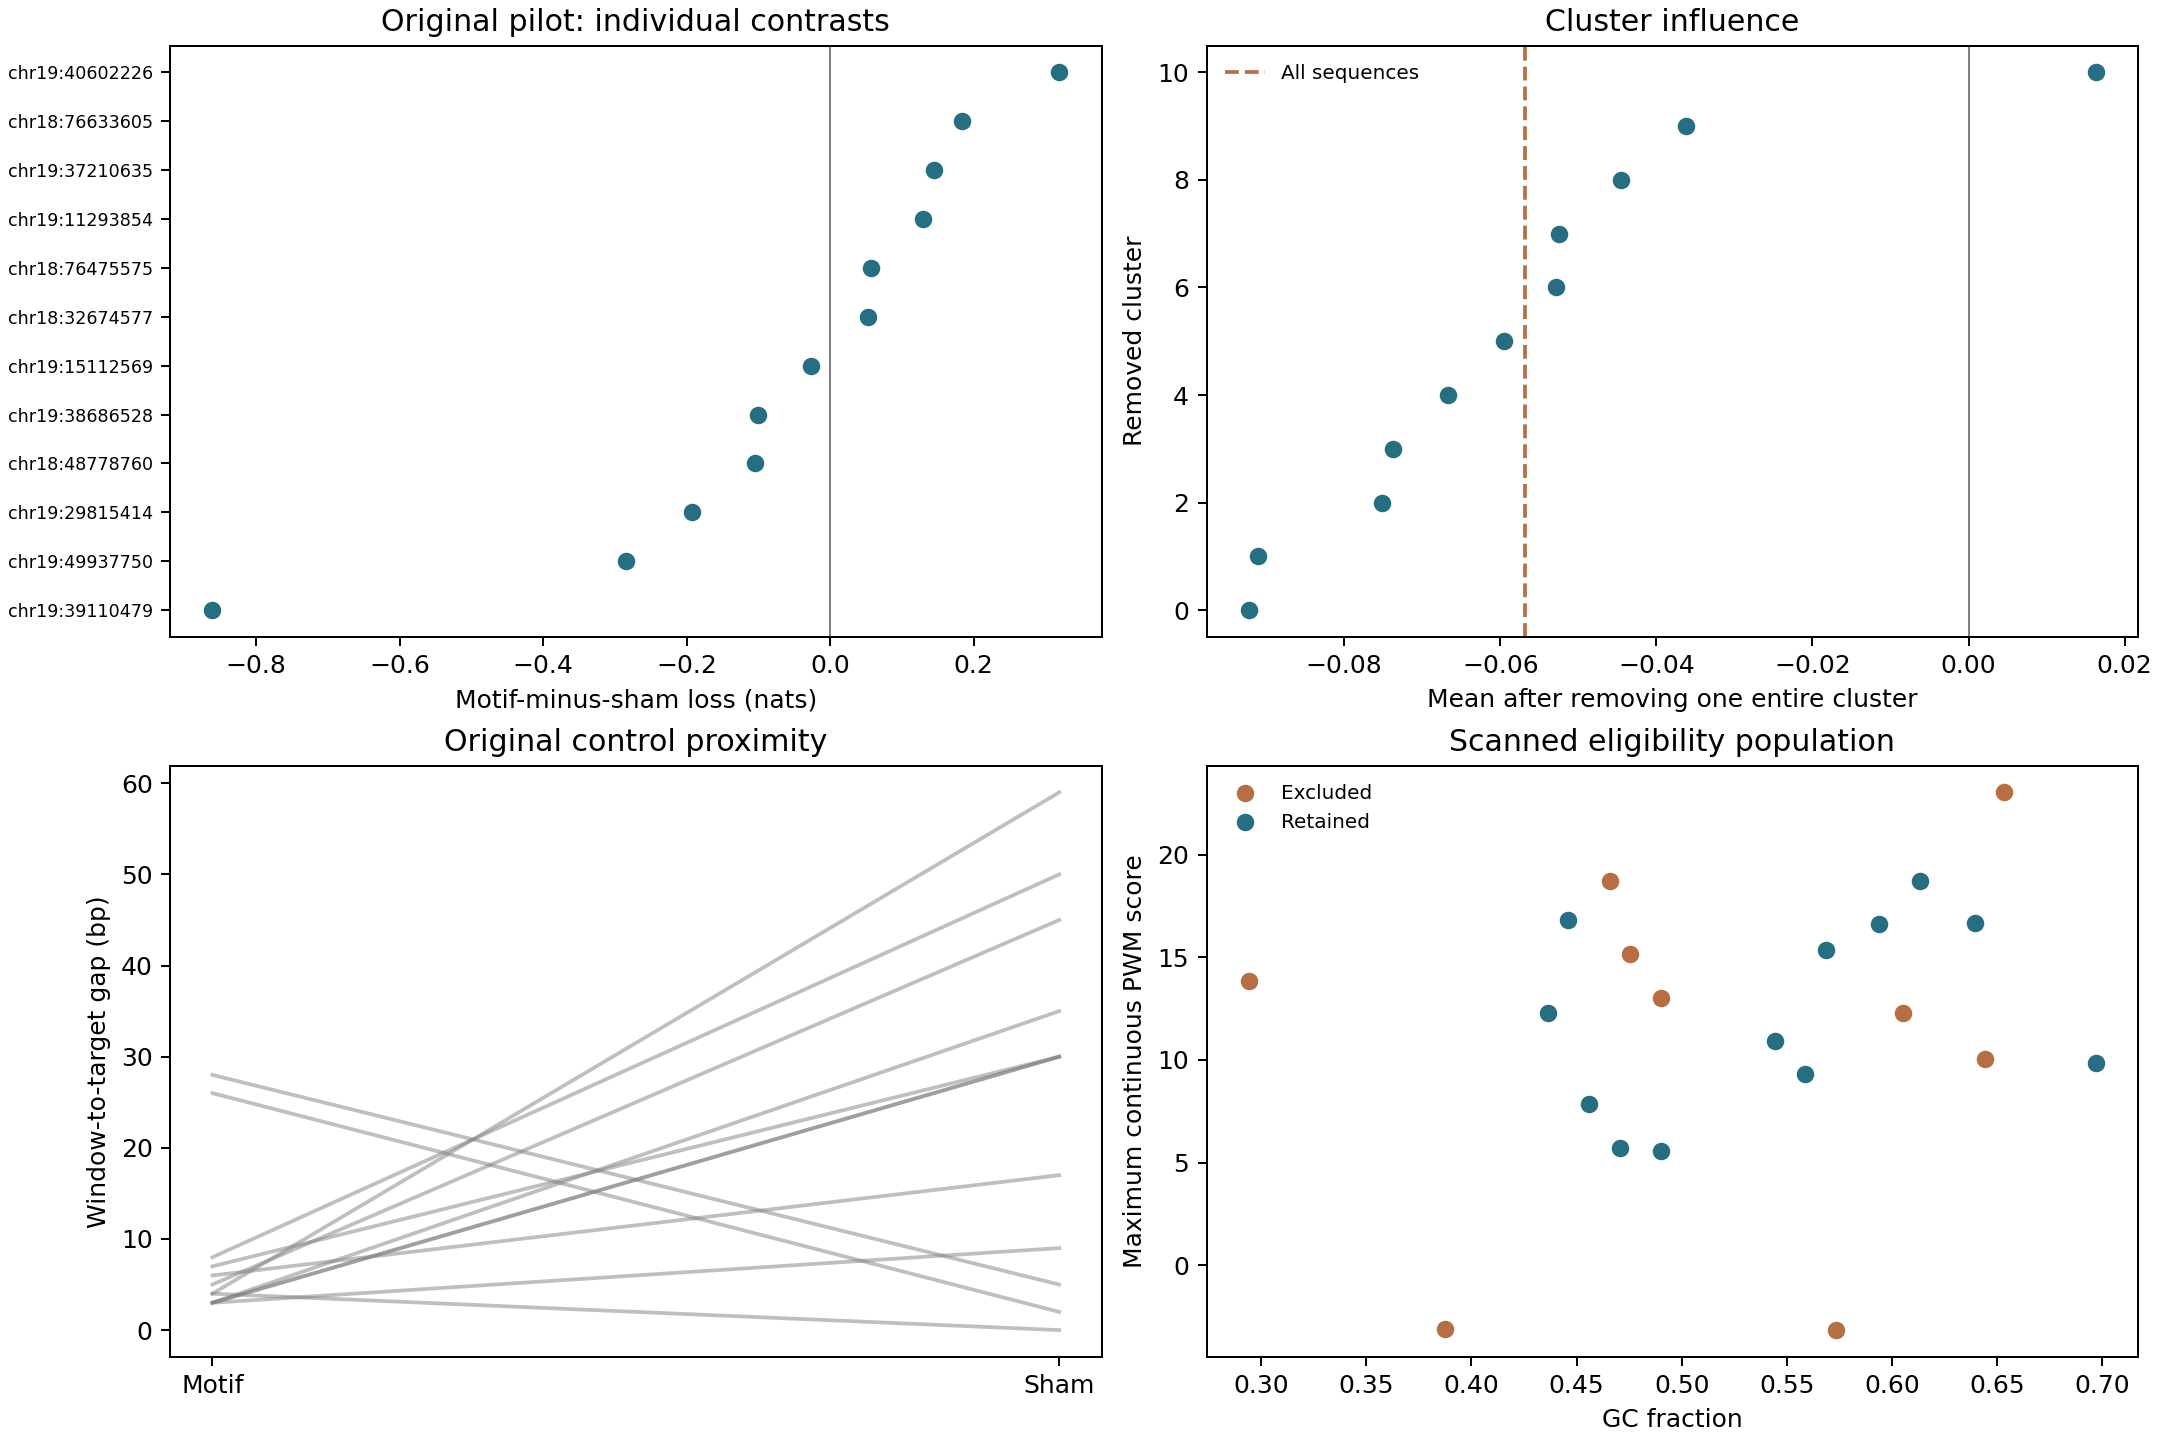
\includegraphics[width=\linewidth]{../results/native_followup/pilot_diagnostics.png}
\caption{Discovery-pilot geometry, eligibility and cluster influence. Leave-cluster-out estimates remove every sequence in the omitted genomic cluster; changing signs indicate sensitivity to membership.}
\label{fig:pilot-diagnostics}
\end{figure}
\begin{figure}[t]
\centering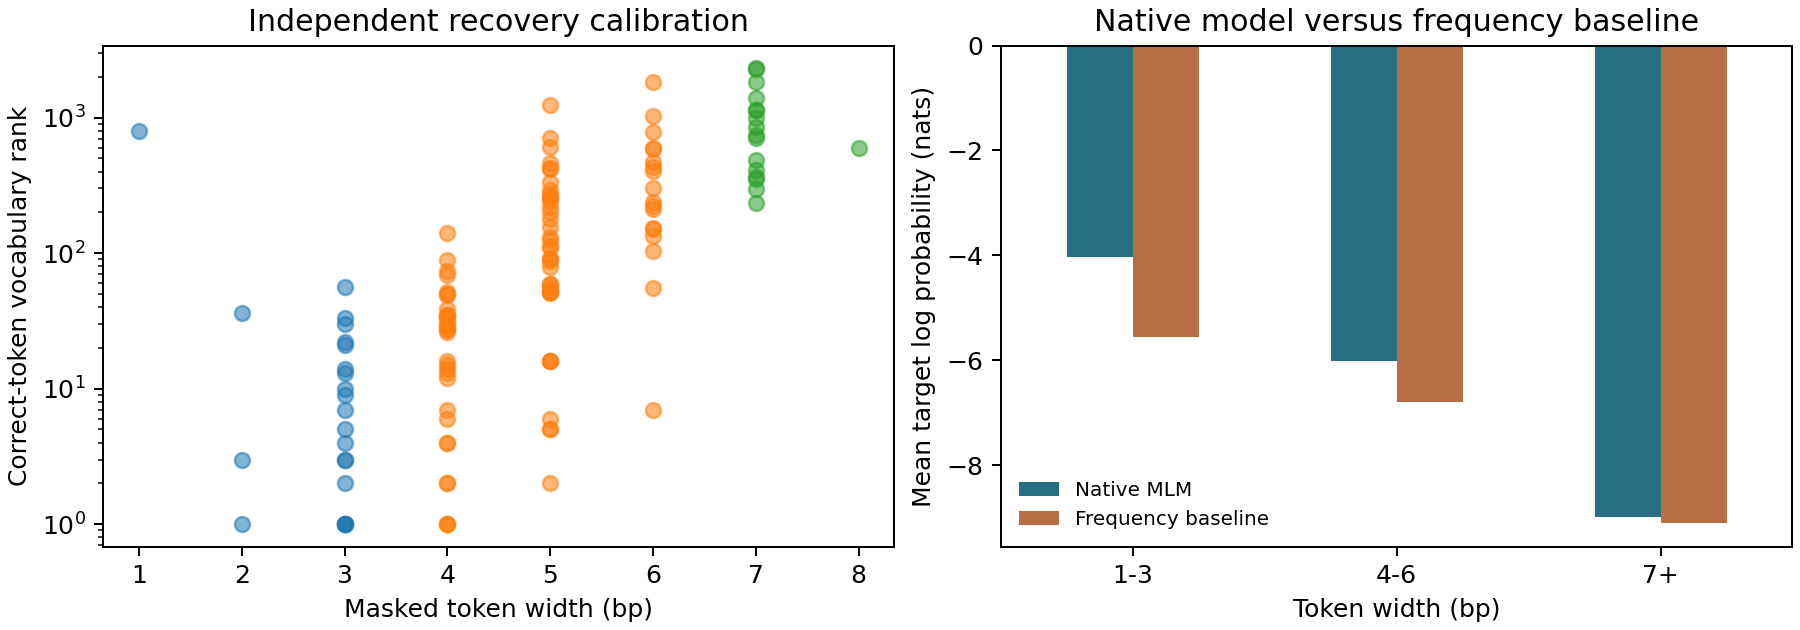
\includegraphics[width=.9\linewidth]{../results/native_followup/recovery_calibration.png}
\caption{Independent masked-token recovery on 128 fixed chromosome 16/17 windows. Vocabulary rank and log probability depend on token width; comparison uses a smoothed token-frequency baseline from chromosomes 14/15. This calibrates recovery competence without testing motif-specific sensitivity.}
\label{fig:recovery-calibration}
\end{figure}
\paragraph{Donor control feasibility.}
For a two-base GT-to-TG edit, a non-motif sham with the same width and transition multiset must change TG to GT, which creates a prohibited new hit. The resulting donor exclusion concerns the feasibility of this strict control design, rather than absence of a donor mechanism. A wider-context donor control is outside these intervention results.
\FloatBarrier
\section{Interpretation and limitations}
The native extension is gated on endpoint feasibility. Its current masked-flank pilot fails that gate, and its interval is too wide for a precise null. Any revised endpoint is exploratory. A subsequent confirmation would require a fully frozen endpoint, selection and intervention rule, matched controls, eligibility, genomic clustering and a cluster-based power justification on genuinely uninspected inputs. The inspected chromosomes 20/21 cannot provide that confirmation. The recovered GSE81945 study supplement provides 15 heterozygous variants across 13 hg19 loci, with reference alleles verified against hg19. Pooled counts and two adjacent-variant groups limit independent allele inference; no hg38 transfer or biological confirmation is claimed. Natural substitutions require substitution-matched controls, rather than composition-preserving shuffle controls.
Evidence supports frozen decodability, failure of historical CTCF screens, and sequence-level QK and native-attention measurements under matched genomic controls, without identifying native CTCF causality. A validated native pretrained causal target remains unresolved; the added CTCF target is an independently evaluated trained readout. The corrected analyses use different aggregation and a different control population from the historical screens; the assays are not interchangeable. Small selected patching populations and composition-changing corruptions prevent broad causal conclusions. The controlled assays above establish nucleotide correspondence and matched shams for their retained populations, with explicit eligibility exclusions.

The affine QK observation is conditional: if logits for a fixed query equal $a+\gamma s_j$ with $\gamma>0$, softmax preserves score ordering within that sequence. This assumption is not shown empirically. Within-sequence ranking does not imply a cross-sequence motif-present/absent threshold or causal use; we make no stronger layer-1 theorem claim.

The Nucleotide Transformer comparison is excluded because a pinned checkpoint, validated token alignment, and native-attention equivalence were not established. Its stored enrichment ratio is not Spearman correlation. No tokenizer-family ranking or cross-model biological conclusion is supported. Auxiliary OV and sparse-feature artifacts are historical; weak alignment does not show that an alternate circuit is absent.

Intervals concern fixed classifiers and do not resolve labeling errors, pretraining contamination, distant homology or training-seed variability. The added analyses report sensitivity to within-chromosome dependence through transitive genomic blocks. Local membership matches the pinned upstream release, but historical checkpoint provenance and independent label reconstruction remain incomplete. The predictive, held-out TATA, and native-control results use the completed clean CUDA reproduction. Fresh train/test activation caches and CTCF sequence/token files match their historical counterparts byte for byte, and the historical screen conclusion is reproduced. Refitted probe outputs differ slightly across the recorded environments. The clean pipeline completed through recorded resumptions after a loader compatibility repair; a diagnostic traceback timer was removed following a native Python crash. Earlier disk-exhaustion failures and all failed or interrupted attempts are preserved.
\FloatBarrier
\section*{Author declarations}
Arjun VIjay Prakash is the sole author and has reviewed and approved this manuscript. The author received no funding for this work and declares no competing interests. This study analyzes previously available computational and genomic resources; it reports no new participant recruitment or biological sample collection.
\clearpage\bibliographystyle{plainnat}\bibliography{references}\end{document}
